\documentclass[12pt,titlepage]{scrartcl}
\usepackage[ngerman]{babel}
\usepackage[utf8]{inputenc}
\usepackage{color}
\setkomafont{disposition}{\normalfont\bfseries}
\usepackage[a4paper,lmargin={3cm},rmargin={3cm},
tmargin={2.5cm},bmargin = {2.5cm}]{geometry}
\usepackage{graphicx}
\usepackage{amssymb}
\usepackage{amsthm}
\usepackage{caption}
\usepackage{float}
\usepackage{cite}
\usepackage{hyperref}

\begin{document}
	\begin{titlepage}
		\title{Exposé \\ \glqq Synchronisierung von analogen und digitalen Scrum-Boards\grqq{}} 
		\subtitle{Praxisprojekt}
		\author{Alexander Strutz \vspace{0.5cm}\\ Betreuer: 
		Prof. Dr. Matthias Böhmer,\\Oliver Blum}
 		\date{26. Februar 2019}
		\maketitle
	\end{titlepage}
	\newpage
	\noindent \textbf{Kontext} \\
	In 63\% der deutschen IT-Firmen und Agenturen werden laut Umfrage der Hochschule Koblenz agile Arbeitstechniken wie das Framework „Scrum“ verwendet \cite{hskob}. Während sich agile, auch leichtgewichtig genannte, Prozesse an dem „Agilen Manifest“ orientieren, ist für Scrum ein Satz an Grundregeln und Vorgehensweisen definiert. \\
So sind selbstorganisierte Teams ebenso ein Bestandteil wie ein Team-Board, an dem die Aufgaben (Stories genannt) in Form von Zetteln hängen. Stories können drei verschiedene Status annehmen: ''To Do'', ''In Work'' und ''Done''. Durch einen täglichen Termin innerhalb des Teams, dem sogenannten Daily, wird der aktuelle Status der Stories erläutert und entsprechend auf dem Board verschoben \cite{guide}. \\
\begin{figure}[H] 
  				\centering
    			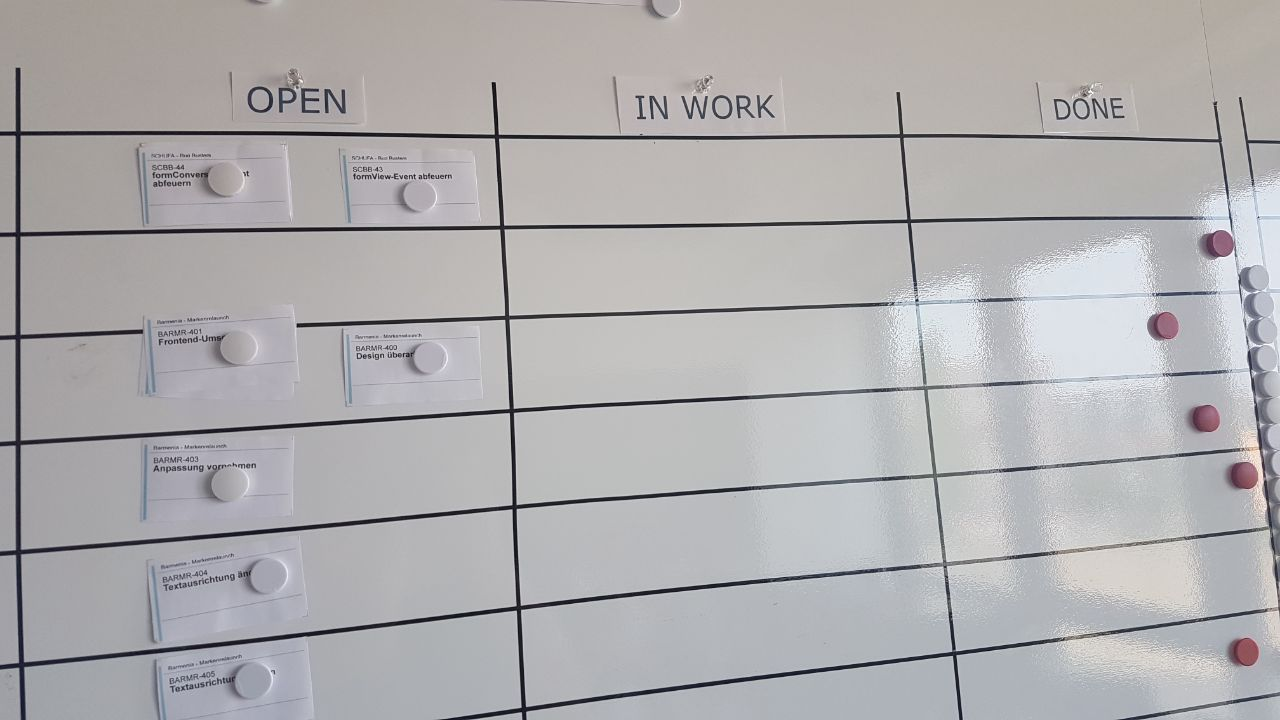
\includegraphics[height=0.3\textheight]{physicalBoardNear}
  				\caption{Beispiel eines physischen Boards}
  				\label{fig:ANHphysKernNear}
			\end{figure}
\noindent Parallel dazu nutzen viele Firmen digitale Ticketsysteme, wie z.B. JIRA. Der Vorteil dieser Systeme ist die Sichtbarkeit des Fortschrittes. Während Kunden das physische Board des Teams nicht immer sehen können, sind Systeme wie JIRA dafür ausgelegt sowohl Kunden als auch Dienstleistern einen Überblick über Stories zu geben. Darüber hinaus können im digitalen System auch Anhänge, Zuweisungen, Kommentare und verknüpfte Stories hinterlegt werden. \\ \\
\textbf{Problemszenario und Zielsetzung} \\
Bei dieser Arbeitsweise entsteht das Problem, dass das physische Board und das digitale Ticketsystem nicht synchron gehalten werden können ohne einen zeitlichen Aufwand entstehen zu lassen \cite{sync}. Auch kann es zu Inkonsistenzen zwischen den Boards kommen, falls Teammitglieder vergessen den Status einer Story auf beiden Boards anzupassen. Daher ist das Ziel dieses Praxisprojektes die möglichst automatisierte Synchronisierung dieser Systeme. Es ergibt sich somit die Forschungsfrage: \\
„Wie lassen sich analoge und digitale Scrum-Boards synchronisieren?“
\newpage
\noindent
\textbf{Ressourcen} \\
Um diese Synchronisierung nah an Scrum zu halten, sind der Scrum-Guide und das dahinter stehende ''Agile  Manifest'' die referenzierten Hauptwerke (vgl. \cite{manifest} und \cite{guide}). Darüber hinaus werden weitere Werke und Studien zur Psychologie der Nutzung von analogen und digitalen Anwendungen verwendet, wie beispielsweise ''The pen is mightier than the keyboard'' und ''The progress principle'' \cite{pen}, \cite{progress}. \\
Technologisch wird ein Prototyp aus dem Fachbereich des ''Internet of Things'' angestrebt, welcher über einen HTTP-Server mit dem JIRA, bzw. einer entsprechenden JIRA API kommunizieren kann. Getestet und evaluiert wird der Prototyp im Unternehmen ''kernpunkt'', welches nach Scrum in selbstorganisierten Teams arbeitet.\\ \\
\textbf{Motivation} \\
Angesichts der hohen Nutzung von agilen Methoden besitzt dieses Problem eine besondere Relevanz im Umfeld von IT-Unternehmen und Agenturen. Eine zusätzliche persönliche Motivation ist die Senkung des Papierverbrauchs. Wenn die Stories auf Papier durch IoT-Geräte ausgetauscht werden, schont dies auf lange Sicht die Umwelt. \\
Prädestiniert ist dieses Problem für Medieninformatiker, da es darum geht ein analoges Medium mit einem digitalen Medium mit den Werkzeugen der Informatik zu synchronisieren. Die Lösung dieses Problems muss nicht nur eine technische Qualität aufweisen, sondern auch ein alltagstaugliches Medium und Kommunikationsmittel darstellen.\\ \\
\textbf{Struktur und Planung} \\
Im Mittelpunkt des Praxisprojektes steht die Entwicklung eines Prototypen zur Erfüllung verschiedener Anforderungen. Zu Beginn werden diese definiert. Daraufhin werden verschiedene technologische Ansätze recherchiert und abgewogen. Nach der Entscheidung geeigneter Technologien, sowohl für die Hardware am Board als auch für die Software zur Kommunikation mit dem Ticketsystem wird eine Architektur entwickelt, die auf diese Technologien abgestimmt ist. Im Rahmen dieser Architektur werden die Anforderungen realisiert und zu einem zusammengehörigen System vervollständigt. Schlussendlich wird das System anhand der selbst definierten Anforderungen getestet.\\ \\
\textbf{Setup, Abhängigkeiten und Meilensteine} \\
Der Prototyp wird in Kooperation mit der kernpunkt Digital GmbH aus Köln umgesetzt mit Oliver Blum, einem der zwei Geschäftsführer, als Betreuer vor Ort. Die benötigten Ressourcen, wie Bauteile, Speicher, Server und Software, wie z.B. JIRA, wird vom Unternehmen gestellt. Prüfer ist Prof. Matthias Böhmer. Die Implementation erfolgt im Unternehmen an den dortigen Scrum Boards und kann an den dortigen Teams getestet werden. \\
In der darauffolgenden Bachelorarbeit wird der entwickelte Prototyp erweitert zu einem alltagstauglichen System. Hierbei soll der Prototyp im Unternehmen evaluiert werden. Aus den Rückmeldungen der Teams werden neue Anforderungen abgeleitet, die implementiert werden. Abschließend wird das System erneut evaluiert und mit der Ausgangssituation verglichen. \\
\begin{table}[H]
\centering
\caption{\textbf{Meilensteine des Praxisprojekts}}
\begin{tabular}{|c|l|}
\hline
\multicolumn{1}{|l|}{\textbf{Datum}} & {\textbf{Artefakt}} \\ \hline
26.02.2019                                 & Expose fertiggestellt \\ \hline
11.03.2019                                 & Anforderungen definiert\\ \hline
25.03.2019                                       & Architekturmodell und Technologieentscheidung getroffen \\ \hline
22.04.2019                                       & Anforderungen umgesetzt                                  \\ \hline
29.04.2019                                       & PP dokumentiert und Anforderungen geprüft                                \\ \hline
30.04.2019                                       & PP abgegeben\\ \hline
\end{tabular}
\end{table}
\noindent \textbf{Ergebnis und Verwertung} \\
Das Ergebnis dieser Arbeit soll ein Protoyp eines Systems sein, welches physische Boards um digitale Komponenten erweitert. Dieser Prototyp soll den organisatorischen Aufwand von Product Owner und Scrum Master reduzieren und somit ein effizienteres Arbeit ermöglichen. Weitergehend kann ein Produkt entwickelt werden, welches agiles Prozesse weiter unterstützt. 
Ein solches Produkt kann als Grundlage zur Entwicklung weiterer „Brückensysteme“ dienen, die die Verzahnung von digitalen und analogen Boards weiter vorantreiben würden. Ein positiver Nebeneffekt wäre die Verbesserung der Kommunikation innerhalb des Teams durch ein stets aktuelles Board. \\
Die Relevanz dieses Themas wird verdeutlicht, wenn man Studie ''Status Quo Agile 2016/2017'' betrachtet. Demnach nutzen 85\% der agilen Unternehmen Scrum \cite{hskob}. Diese Unternehmen können durch die Ergebnisse dieser Arbeit die Qualität ihrer Teams, sowie ihren Umsatz steigern. Somit entstehen auch wirtschaftlich wertvolle Erkenntnisse. An diesen Erkenntnissen sind dementsprechend Personen in leitenden Positionen interessiert. Aber auch Scrum Master, Product Owner und Entwickler profitieren von einem Prototyp und einer Weiterentwicklung. Ferner können diese Boards zur Weiterentwicklung und auf Messen zu Agilität in Unternehmen genutzt werden. 
\newpage

\bibliography{Expose}
 		\bibliographystyle{unsrt}
\end{document}
